\documentclass[22pt, a4paper]{report}

\usepackage[utf8]{inputenc}
\usepackage[T1]{fontenc}
\usepackage[francais]{babel}
\usepackage{verbatim}
\usepackage{color}
\usepackage{hyperref}
\usepackage{lmodern}
\usepackage{graphicx}
\usepackage{caption}
\usepackage{subfig}
\usepackage[subfigure]{tocloft}
\usepackage[french,boxruled,lined]{algorithm2e}
\usepackage[a4paper,vmargin={20mm,20mm},hmargin={30mm,20mm},includeheadfoot]{geometry}
\usepackage{listingsutf8}
\lstset{
language=c,
breaklines=true,
inputencoding=utf8/latin1
}

% Paquets requis par Doxygen
\usepackage{calc}
\usepackage{doxygen}
\usepackage{makeidx}
\usepackage{multicol}
\usepackage{multirow}
\usepackage{textcomp}
\usepackage[table]{xcolor}
\usepackage{ifpdf}
%\usepackage[pdftex,pagebackref=true]{hyperref}

% Commande pour Doxygen
\providecommand{\clearemptydoublepage}{%
  \newpage{\pagestyle{empty}\cleardoublepage}%
}

\SetKwInput{Var}{Variables}
\SetKwInput{Data}{Données}
\SetKwInput{Result}{Résultat}
\SetKwIF{Si}{Ssi}{Sinon}{Si}{alors}{sinon si}{sinon}{finsi}
\SetKwFor{Pour}{Pour}{faire}{finpour}
\SetKwFor{tq}{Tant que}{faire}{fintq}
\SetKwRepeat{Repeter}{Répéter}{jusqu'à}
\SetKwFor{ForEach}{Pour chaque}{faire}{finpour}
\SetKw{Renvoyer}{Renvoyer}
\SetKw{De}{de}
\SetKw{A}{à}

\title{\textbf{Projet Link-Pix}}
\author{
  \href{mailto:ambroise.bernhardt@etud.univ-montp2.fr}{Ambroise Bernhardt - ambroise.bernhardt@etud.univ-montp2.fr}\\
  \href{mailto:florian.galinier@etud.univ-montp2.fr}{Florian Galinier - florian.galinier@etud.univ-montp2.fr}\\
  \href{mailto:adrien.plazas@etud.univ-montp2.fr}{Adrien Plazas - adrien.plazas@etud.univ-montp2.fr}\\
  \href{mailto:chloe.tronc@etud.univ-montp2.fr}{Chloé Tronc - chloe.tronc@etud.univ-montp2.fr}
}
\date{}

\begin{document}

\maketitle

\begin{abstract}
Ce rapport est le compte rendu du projet Link-Pix exécuté par les auteurs et proposé par Philippe Janssen pour l'unité d'enseignement GLIN405 Projet Informatique du quatrième semestre du parcours Licence Informatique de la Faculté de Sciences de Montpellier en 2012-2013.
\end{abstract}

\chapter*{Remerciements}
Nous remercions tout particulièrement Philippe Janssen pour nous avoir brillament encadré et soutenu tout le long de la réalisation de ce projet.

\tableofcontents

\chapter{Introduction}

Lorsqu'un programme nécessitait un stockage des données complexes et ordonnées, son créateur décidait de la manière dont les données étaient organisées en mémoire, permettant donc de définir le comportement spécifique de son application au moment de la lecture de données enregistrées. C'est dans ce contexte que le problème de la communication de données entre deux applications ou plus s'est posé. En effet, chaque programme avait sa manière d'interpréter des données stockées et les organisait de manière spécifique, la communication directe n'était donc pas possible, il fallait donc trouver un moyen intermédiaire afin de convertir les données destinées à une application vers un format lisible par un autre programme. Sauf que créer cet intermédiaire engendrait d'important coûts en termes de développement, d'autant plus que si une nouvelle application avait besoin de ces données, il aurait à nouveau fallu recréer un intermédiaire spécifique.
\paragraph{}

C'est ainsi que le principe d'une structure de données commune a émergé et que les langages de balisage se sont popularisés, permettant en plus d'avoir une structure stricte et normalisée. XML ou "Extensible Markup Language" fait partie de ces langages. Ce langage a de plus pour caractéristique d'être, d'où son nom, extensible, c'est-à-dire que les désignations des balises ne sont pas fixes, elles sont définies spécifiquement pour les données sauvegardées. Pour finir, il est possible de définir un XML Schema afin de restreindre et de contrôler la structure même du document XML, afin de vérifier s'il est écrit de la bonne manière et valide en termes d'organisation.
\paragraph{}

Le projet qui nous a été confié consiste à concevoir et à développer une application faisant office d'éditeur XML permettant donc à n'importe quel utilisateur qui utilisera l'interface de créer ou de modifier un document XML à sa guise, le tout en conservant le respect des normes dictées par le standard XML, incluant donc tout le processus de validation des données.
\paragraph{}

Après avoir exposé l'analyse menée pour étudier le projet même, ses spécifications et ses besoins, nous présenterons le rapport d'activité rendant compte des méthodes de travail que nous avons utilisées pour mener à bien ce projet. Le rapport technique décrit les choix de conception ainsi que des extraits plus pratiques, expliquant des portions de code. Et enfin, après avoir présenté le manuel d'utilisation de l'application, nous conclurons en exposant des perspectives d'amélioration du logiciel.
\chapter{Organisation du projet}

  \section{Organisation du travail}

    \subsection{Réunions de travail}
Une réunion hebdomadaire était tenue tous les mardis, d'abord à 13h15, rapidement décalée à 11h20. Certaines réunions exceptionnelles ont pû être rajoutées le jeudi.

    \subsection{Répartition des tâches}
Les tâches étaient assignées au dévouement ou, si certaines tâches n'étaient pas assignées et que des personnes ne s'étaient pas dévouées, par l'encadrant.

    \subsection{Planification du développement}
On peut analyser la méthode de développement utilisée de la manière suivante :
\begin{itemize}
	\item analyse globale du problème~;
	\item analyse des structures de données nécessaires à la résolution du problème~;
	\item implémentation des structures et de leurs fonctions associées~;
	\item analyse en profondeur du problème et écriture des algorithmes nécessaires à sa résolution~;
	\item implémentation des algorithmes en s'appuyant sur les structures déjà implémentées~;
	\item construction de l'application finale à partir des briques logicielles implémentées.
\end{itemize}

    \subsection{Élection d’un chef de projet}
Aucun chef de projet n'a été élu, les décisions ont été prises lors des réunions, où tout le monde pouvait faire des propositions qui étaient alors débattues.
Le groupe de travail était suffisamment restreint pour qu'un tel système fonctionne.

    \subsection{Gestion du groupe d’étudiants}
La gestion du groupe s'est faite par courriel, lors des réunions et lors de rencontres hors du cadre du projet.
Elle s'est avérée compliquée et de nombreux problèmes de communication et tout particulièrement de non comunication et d'absentéisme sont apparus et ont retardé le projet.

  \section{Choix des outils de développement}

    \subsection{Choix du langage}
Le langage initialement proposé par notre encadrant était le C. Ce langage étant le mieux connu de toute l'équipe, il avait alors un avantage subjectif mais réel.

Il s'avère que le C répondait en outre assez bien aux besoins du projet, qui n'a nécessité que des structures de données assez simples.

La question posée a été celle de la version du langage à utiliser : C89 ou C99 ?
Au final le C89 a été choisi, afin de forcer l'équipe à utiliser un langage plus strict.

    \subsection{Choix de l'éditeur}
Le C étant un langage permettant un choix extrêmement souple d'éditeurs, il a été décidé de ne pas associer le projet à un éditeur particulier et de favoriser l'utilisation d'outils simples.
Ainsi le choix d'un simple éditeur de texte et d'un émulateur de terminal a été fait par la majorité, sinon la totalité, des membres de l'équipe.

    \subsection{Choix du compilateur}
GCC est le compilateur C utilisé par tous à la faculté, de plus certains membres de l'équipe sont attachés aux outils GNU, ainsi son choix a été fait sans se poser de questions particulières.

Le choix a été fait sur le tard d'en activer les options \verb|--ansi| et \verb|--pedantic| pour plus de rigueur dans le code.

    \subsection{Choix du débogueur}
Pour des raisons similaires à celles du choix du compilateur, GDB a été choisi pour nos besoins de déboguage.

    \subsection{Choix du gestionnaire de projet et du gestionnaire de versions}
Le service informatique de la faculté a mis à disposition des étudiants et professeurs un service d'hébergement et de gestion de projet utilisant GitLab aux alentours du démarrage du projet.
Il a rapidement été décidé de l'adopter, ainsi Git a été choisi comme gestionnaire de version car c'est celui utilisé par GitLab.

    \subsection{Choix des outils d'analyse}
Aucun outil d'analyse n'a été utilisé.

    \subsection{Choix des outils de documentation}
Concernant la documentation du code, Doxygen a été proposé par notre encadrant et a été accepté par les membres de l'équipe.
Quant au rapport, le choix de \LaTeX a été fait car il permet de modulariser et de simplifier le travail à plusieurs sur un document par rapport à des outils de traitement de texte plus classiques utilisant un format de fichier binaire et monolithique.

\chapter{Analyse du projet}
\section{Contexte}
Le langage Extensible Markup Language ou XML est utilisé à des fins de stockage de données, et est structuré par un schéma qui lui est associé, il permet de definir la structure et le type de contenu du document, en plus de permettre de verifier la validité du document.
\paragraph{}

Généralement, les fichiers XML sont générés par un programme quelconque dans le but d'échanger des données ou de les stocker, XML faisant office de plateforme commune. Mais on peut également utiliser un éditeur de texte basique pour créer de toute pièce un document XML, avec des fonctionnalités propre à un éditeur de texte, sans fonctionnalités spécialement prévues pour XML.
\paragraph{}

C'est dans ce contexte que des solutions logicielles d'éditeur XML ont vu le jour : un éditeur de texte qui possède des fonctionnalités permettant une écriture d'un fichier XML beaucoup plus rapide et efficace, le tout avec un contrôle des erreurs.
	
\section{Analyse de l'existant}
Plusieurs solutions sont déjà proposées, certaines étant payantes et d'autres sont gratuites et open source. L'objectif est ici de fournir une solution similaire aux autres logiciels.
\paragraph{}

En se basant sur le logiciel le plus pertinent d'après les recherches autour du sujet "xml editor", le logiciel oXygen XML Editor semble être le plus présent et utilisé. C'est une solution logicielle contenant deux principaux outils : XML Developer et XML Author. Le tarif pour le package complet de XML Editor est au prix de 488\$ ou 19\$ par mois là ou chaque outil coûte à l'unité 349\$, ce qui en fait un logiciel très onéreux. L'entreprise propose cependant une version d'essai de 30 jours pour tester le logiciel. Le programme propose un nombre très important de fonctionnalités dans le but d'être utilisable à la fois par un développeur qui connaît déjà le langage et qui voudrait optimiser la saisie de fichiers XML et par un novice de XML avec un système d'assistants de création de documents.
\paragraph{}

La figure \ref{oxygen} expose par exemple une vue spéciale du document sous forme de tableur, permettant une modification beaucoup plus aisée des attributs des nœuds.

%\newpage
\vfill

\begin{figure}[H]
      \centering
      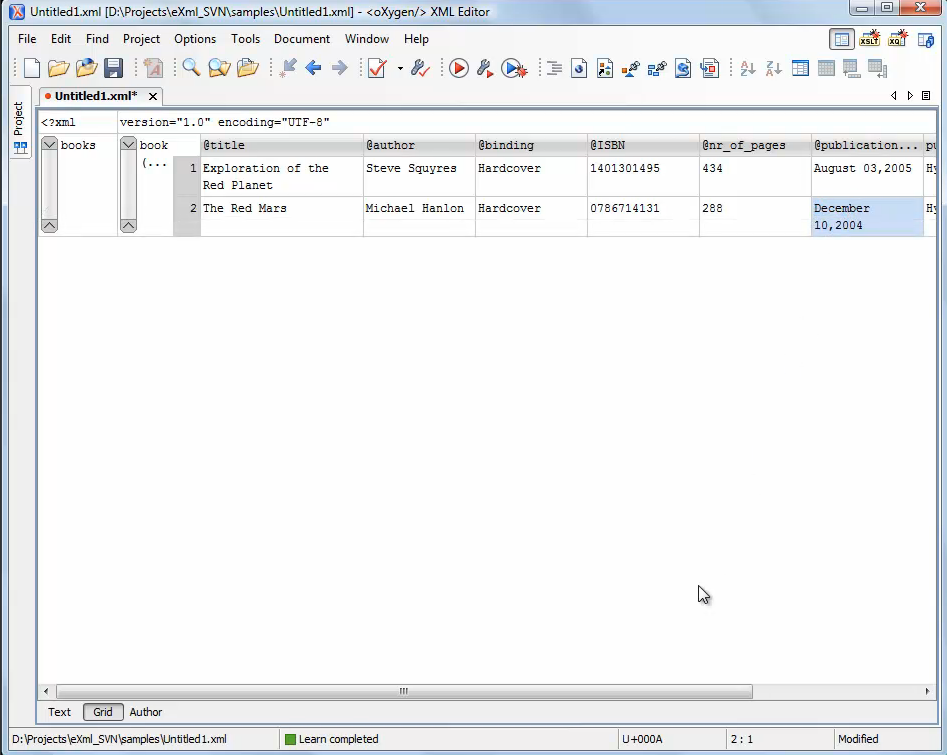
\includegraphics[scale=0.5]{images/analyse-oxygen1.png}
      \caption[Maquette d'interface]{Maquette qsdqdsqsdd'interface.}
\end{figure}


\vfill
\clearpage

\begin{figure}[h!]
\begin{minipage}[b]{\linewidth}
\centering 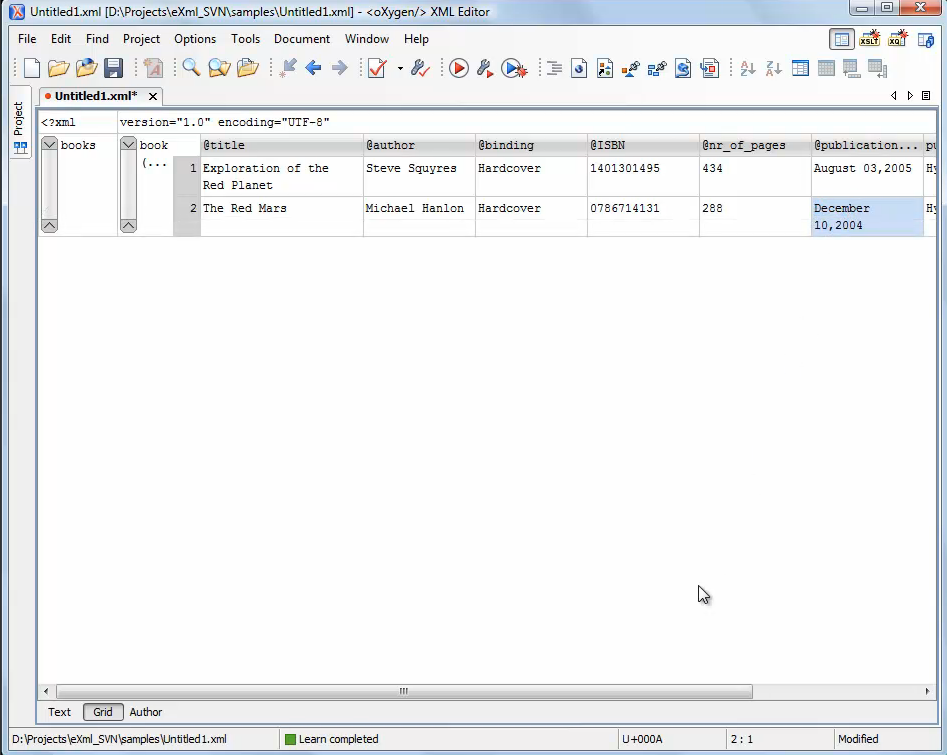
\includegraphics[scale=0.5]{images/analyse-oxygen1.png}
\caption{Exemple de vue avec Oxygen}
\label{oxygen}
\end{minipage}
\end{figure}


\section{Analyse des besoins fonctionnels}
L'objectif du projet est de développer un éditeur XML multi-vues avec différentes fonctionnalités.
\paragraph{}
Les fonctionnalités liées à un éditeur de texte simple devront être présentes : la possibilité de saisir manuellement au clavier l'intégralité du fichier, la création et la sauvegarde du fichier à manipuler ainsi que l'ouverture d'un fichier déjà existant dans le but de le modifier.
\paragraph{}
Des fonctionnalités d'éditeur de texte avancées seront aussi présentes : coloration syntaxique et indentation automatique du code permettant ainsi une lisibilité claire des fichiers manipulés et une autocomplétion du code écrit permettant un gain de temps au cours de la frappe.
\paragraph{}
Pour finir, l'éditeur proposera des fonctionnalités spécifiques au langage XML : validation syntaxique du fichier, vue arborescente du fichier XML avec possibilité de modification des données via cette vue et ajout d'un schéma sur lequel la validation se basera.
\paragraph{}	
La figure \ref{maquette_interface} expose la maquette d'interface de l'éditeur avec chacune des parties annoncées : à gauche la vue arborescente affichant chaque nœud de l'arbre formé par les données, à droite l'éditeur de texte avec toutes ses fonctionnalités associées et en haut la barre d'outils avec la gestion de fichiers (nouveau fichier, ouvrir, sauvegarder) ainsi que la gestion du schéma.

\begin{figure}[h!]
\begin{minipage}[b]{\linewidth}
\centering 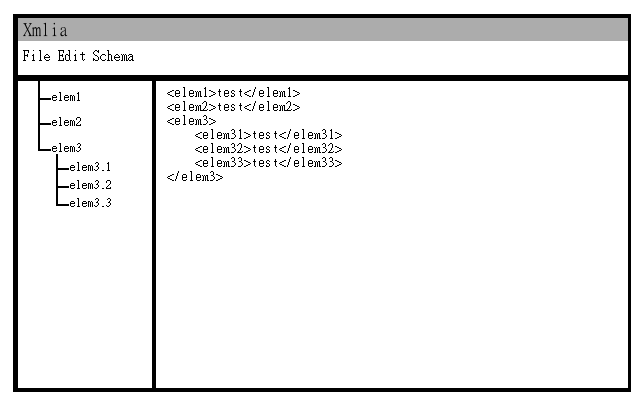
\includegraphics[scale=0.5]{images/analyse-maquette.png}
\caption{Maquette d'interface}
\label{maquette_interface}
\end{minipage}
\end{figure}
	
\section{Analyse des besoins non fonctionnels}
\subsection{Spécifications techniques}
Le programme devra permettre de créer des fichiers XML structurés avec un respect des normes de balisage et, s'il est défini, du schéma de données. De plus, les données saisies ou modifiées à l'aide de l'éditeur doivent rester exploitables, sans corruption du fichier original. Pour terminer, l'éditeur aura à répondre dans des durées acceptables et de manière stable, dans la mesure où la taille et la complexité des données restent raisonnables.
		
\subsection{Contraintes ergonomiques}
Le logiciel devra être suffisamment simple pour qu'un utilisateur connaissant déjà le fonctionnement du XML puisse l'utiliser sans être bloqué par une courbe d'apprentissage trop élevée. On utilisera pour cela des icônes claires et des textes explicatifs.
\paragraph{}
Un utilisateur avancé pourra augmenter sa productivité en utilisant les raccourcis clavier disponibles et pourra gagner de temps en réduisant les transitions souris/clavier.

\chapter{Définition des structures}


\section{Les structures}
La résolution du problème requiert des structures de données afin de représenter :
\begin{itemize}
\item des coordonnées, représentées par la structure \verb$Coordonnees$ (voir \ref{Coordonnees_8h}) contenant deux entiers $x$, l'abscisse, et $y$, l'ordonnée et permettant de situer une case dans un puzzle ;
\item des indices, représentés par la structure \verb$Indice$ (voir \ref{operationLInd_8h}) contenant la valeur d'une case et sa coordonnée ;
\item un ensemble d'indices représenté par une liste ;
\item un ensemble de coordonnées également représenté par une liste ;
\item l'ensemble des «~cases~» contenant les indices et la liste des voisins possibles pour cet indice ;
\item la grille correspondant à l'image résultat (donnant donc les cases «~noircies~»).
\end{itemize}
Nous avons choisi de représenter ces deux derniers points par une unique structure \verb$TabVoisins$.

\subsection{Les listes chainées}
Nous avons défini deux types de listes chainées : les listes de coordonnées et les listes d'indices.

De façon générale, la liste est composée d'une donnée, sa première valeur, et de l'adresse de l'élément suivant :
\begin{itemize}
\item \verb$ListeCoord$ (voir \ref{operationLCoord_8h}) est donc une liste dont les éléments sont des \verb$Coordonnees$ ;
\item \verb$ListeInd$ (voir \ref{operationLInd_8h}) est, elle, une liste d'\verb$Indice$.
\end{itemize}

Les principales fonctions associées aux listes sont celles de création (constructeur / destructeur), d'insertion et de suppression.
Tout d’abord, la fonction \verb|creerLCoord|, respectivement \verb|creerLInd|, permet la création d’une liste. Elle prend donc en paramètre l'élément tête de la liste ainsi qu'une liste équivalente à la queue de la liste que l'on souhaite créer et pouvant être égale à la liste vide. 
La fonction \verb|detruitLCoord| (respectivement \verb|detruitLInd|) supprime l’intégralité de la liste passée en paramètre.
Les fonctions d’insertion permettent, elles, d’ajouter un élément dans la liste, soit au début soit à la fin.
Enfin, les fonctions de suppression (comme \verb|supprimerpremierLCoord| ou \verb|supprimerdansLCoord|) permettent d’enlever soit le premier soit un élément quelconque de la liste.
Ces deux derniers types de fonctions ne renvoient rien mais modifient des listes.

Ces listes sont définis dans les modules d'opération sur les listes de coordonnées et d'indices situés respectivement dans les fichiers \verb$operationLCoord.h$, \verb$operationLCoord.c$, \verb$operationLInd.h$ et \verb$operationLInd.c$ (voir \ref{graphes-dependance}).

\subsection{Un tableau de voisins}

La structure \verb$TabVoisins$, définie dans les fichiers \verb$TabVoisins.h$ (\ref{TabVoisins_8h}) et \verb$TabVoisins.c$ (voir \ref{graphes-dependance}), est un tableau de cases qui donne pour chaque case sa valeur et la liste de ses potentiels voisins. Pour cela, elle utilise la structure \verb$CaseVoisins$ (voir \ref{TabVoisins_8h}) associant donc :
\begin{itemize}
\item la valeur d'une case, qui peut être : 
	\begin{itemize}
	\item 0 si la case est libre ;
	\item 1 si la case est un indice de valeur 1 ou une case empruntée par un chemin ; 
	\item $n > 1$ si la case est un indice de valeur $n$.
	\end{itemize}
\item sa liste \verb$ListeCoord$ qui est la liste des coordonnées des voisins de la case si celle-ci est un indice de valeur supérieure à 1. 
\end{itemize}
\verb$TabVoisins$ a également en donnée les dimensions du puzzle d’origine.

\begin{figure}[h]
 \centering
 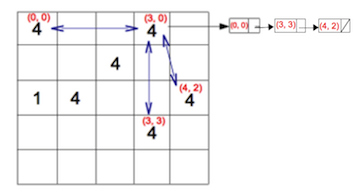
\includegraphics{structures1b}
\caption{Exemple de TabVoisins avec la case $(3, 0)$ qui a la valeur 4 et sa liste de voisins possibles}
\end{figure}

On utilise sur cette structure des fonctions «~basiques~» de création et d'accesseurs :
\begin{itemize}
\item \verb|new_TabVoisins_from_Probleme| qui permet de créer un nouveau TabVoisins représentateur d’un problème donné ;
\item \verb|TabVoisins_getWidth| qui renvoie sa largeur ;
\item \verb|TabVoisins_getHeigth| qui renvoie sa hauteur ; 
\item \verb|TabVoisins_setValeurs| qui permet d'assigner une valeur à une case existante ; 
\item \verb|TabVoisins_getValeurs| qui renvoie la valeur d'une case existante ;
\item \verb|TabVoisins_setVoisins| qui permet de spécifier les voisins potentiels d'une case ; 
\item \verb|TabVoisins_getVoisins| qui renvoie la liste des voisins possibles d'une case.
\end{itemize}

\chapter{Résolution du puzzle Link-Pix}

Le projet a connu différentes étapes de développement. En effet, le solveur étant lui-même découpé en plusieurs parties, nous avons tout d'abord travaillé sur la partie «~mise à jour~» des voisins, avant de passer à la construction des chemins. Nous avons ainsi une partie «~raffinage~» qui a pour objectif de simplifier le problème avant la résolution.

\section{De sous-problème en sous-problème}

\subsection{Modification des voisins}

La première partie du solveur vise à réduire l'ensemble des voisins possibles pour un indice. Ainsi, une coordonnée n'ayant qu'un voisin est, dans le cadre de puzzles qui ont une solution, le seul voisin possible de ce voisin-ci. On peut donc mettre à jour la liste des voisins de cette coordonnée.

Mais les anciens voisins peuvent également se retrouver à ce moment-là avec un unique voisin, il faut par conséquent répercuter la fonction sur eux si c'est le cas.

\begin{algorithm}
  \Data{$c_1$,$c_2$ des coordonnées, avec $c_1$ n'ayant que $c_2$ comme voisin \;
TabVoisin la structure contenant tous les voisins pour chaque coordonnée \;}
\Var{L1, une liste de coordonnées \;}
$L1 \gets TabVoisins\_getVoisins(c_2)$ \;
\ForEach{coordonnée $e$ \De L1}{
  \Si{$e \neq c_1 $}{
    $oterVoisin(c_2,e,TabVoisins)$ \;
    $supprimerdansLCoord(e,L1)$ \;
  }
  $TabVoisins\_setVoisins(c_2,L1)$ \;
}
\caption{affecterVoisin, qui modifie la liste des voisins de $c_2$, avec $c_2$ étant l'unique voisin de $c_1$}
\end{algorithm}

Cette fonction appelle pour chaque coordonnée voisine de $c_2$ la fonction \verb$oterVoisin$. Cette dernière modifie la liste des voisins de $e$ pour supprimer $c_2$, et appelle \verb$affecterVoisin$ si la liste des voisins à la fin est de longueur 1.

\begin{algorithm}
\Data{$c_1$,$c_2$ des coordonnées \;
TabVoisins la structure contenant tous les voisins pour chaque coordonnées \;}
\Var{L1, une liste de coordonnées \;}
$L1 \gets TabVoisins\_getVoisins(c_2) $ \;
$supprimerdansLCoord(c_1,L1)$ \;
$TabVoisins\_setVoisins(c_2,L1)$ \;
\Si{L1 est de longueur 1}{
$affecterVoisin(c_2,$ l'élément de L1 $,TabVoisins)$ \;
}
\caption{oterVoisin, qui supprime $c_1$ de la liste des voisins de $c_2$}
\end{algorithm}

Ainsi, lorsque l'on a une coordonnée $c$ ayant un unique voisin, un appel d'\verb$affecterVoisin$ sur $c$ et son unique voisin se répercutera sur les autres coordonnées «~en contact~» avec ce couple-là. On peut ainsi espérer isoler de la sorte des couples de coordonnées, simplifiant ainsi le problème.

Ces fonctions se situent dans le module «~Mise à jour des voisins~» (fichiers \verb$majVoisins.c$ et \verb$majVoisins.h$) du programme (voir \ref{graphes-dependance}).

\subsection{Existence d'un chemin}

Un deuxième algorithme nous permettant de réduire la liste des voisins possibles est l'algorithme qui teste pour deux coordonnées données, supposées voisines, s'il existe un chemin entre ces deux. Ainsi, si aucun chemin n'existe, on peut en déduire que ces deux coordonnées ne sont en réalité pas voisines.

\begin{algorithm}[H]
  \Data{$c_1$, $c_2$ des coordonnées \;
    $d$ la distance qui doit être parcourue entre $c_1$ et $c_2$ \;
    TabVoisins la matrice contenant les chemins et les indices \;
    L une liste de coordonnées contenant les cases déjà parcourues \;}
  \Result{Le booléen qui vaut Vrai s'il existe un chemin.}
  \Var{L1, une liste de coordonnées \;
    $b$, un booléen \;}
  \Si{$NON(c_1 \in L)$}{
    $L \gets creerListe(c_1,L)$ \;
    $L1 \gets $Liste des cases adjacentes de $c_1$ \;
    \eSi{$d = 2$}{
      \Renvoyer $c_2 \in L1$ \;
    }
        {
          \Tq{NON $b$ ET $L1 \neq NULL$ ET $L1->info$ n'est pas occupée}{
            $b \gets existeChemin(L1->info,c_2,d-1,TabVoisins,L)$ \;
          }  
          \Renvoyer b \;
        }
  }
  \caption{existeChemin, qui teste s'il existe un chemin entre $c_1$ et $c_2$}
\end{algorithm}

Cet algorithme s'appelle de façon récursive et teste tous les chemins possibles, sans repasser deux fois par la même case.

La condition d'arrêt de cet algorithme est dans le cas où on a un chemin à parcourir de longueur 2. Dans ce cas-là, on teste si les cases sont adjacentes. Si ce n'est pas le cas, on progresse comme indiqué dans la partie analyse, en se déplaçant sur les cases adjacentes et en testant s'il existe un chemin de longueur $d-1$.

On pourra ainsi réduire la liste des coordonnées voisines possibles grâce à cette fonction de «~tamisage~», avant de passer à la partie construction.

\subsection{Construction du début d'un chemin}

La construction d'un chemin, ou plus «~simplement~» du début d'un chemin, peut permettre d'éliminer de nouvelles possibilités pour les listes de voisins possibles.

Ainsi, un chemin, même incomplet, permet la progression de la résolution du problème. L'algorithme que nous avons écrit est un algorithme récursif, qui écrit un morceau de chemin et qui, s'il le peut, le complète au fur et à mesure. On a ainsi la fonction qui construira les chemins, mais aussi une fonction qui permettra de «~raffiner~» les listes de voisins.

\begin{algorithm}[H]
  \Data{$c_1$, $c_2$ des coordonnées qui sont uniques voisines l'une de l'autre \;
    $d$ la distance qui doit être parcourue entre $c_1$ et $c_2$ \;
    TabVoisins la matrice contenant les chemins et les indices \;}
  \Result{Un booléen valant Vrai si la construction du chemin a progressé, Faux sinon.}
  \Var{L1, une liste de coordonnées \;
    $s$, un entier \;
    $c$, une coordonnée \;}
  \eSi{$d = 2$}{
    Mettre à jour la grille avec 1 comme nouvelle valeur pour $c_1$ et $c_2$ \;
    \Renvoyer Vrai \;
  }
  {
    $s \gets 0$ \; 
    $L \gets$ Liste des cases adjacentes joignables \;
    \ForEach{coordonnées $e$ \De L}{
      \Si{existeChemin($e$,$c_2$,TabVoisins,NULL)}{$s \gets s+1$ \;
      $c \gets e$ \;}
    }

    \eSi{$s = 1$}{
      Mettre à jour la grille avec 1 pour $c_1$, et $d-1$ pour $c$ et $c_2$ \;
      $consChemin(c,c_2,d-1,TabVoisins)$ \;
      \Renvoyer Vrai \;
    }
        {
          \Renvoyer Faux \;
        }
  }
  \caption{consChemin, qui construit le début d'un chemin (si possible) entre $c_1$ et $c_2$}
\end{algorithm}

Cette fonction va s'arrêter si elle arrive dans le cas de deux indices adjacents et de chemin 2, ou dans le cas où il existe plus d'un début de chemin entre $c_1$ et $c_2$.
S'il n'existe qu'un seul début de chemin possible, elle va alors construire ce début de chemin. Elle va ensuite se positionner sur ce début de chemin, via l'appel récursif, et tenter à nouveau de construire un morceau de chemin.

On pourra aussi appeler cette fonction dans l'autre «~sens~». Car, en effet, il est possible que l'on ne puisse pas construire de morceau de chemin d'une coordonnée vers l'autre, mais que ce soit possible dans l'autre sens.

\section{Solveur}
  
Le solveur en lui-même est une succession d'appel sur les fonctions précédentes. On va ainsi «~tamiser~» le problème, tenter de voir si l'on a alors des chemins possibles, puis re-tamiser le problème, et ainsi de suite jusqu'à ce que la solution apparaisse. La structure globale du solveur sera alors :

\begin{algorithm}[H]
  \Tq{le problème n'est pas résolu}{
    Tamiser le problème \;
    Construire des morceaux de chemins \;
  }
  \caption{Structure globale du solveur}
\end{algorithm}

La boucle principale se décomposera ainsi en deux sous-parties, appelant chacune des fonctions décrites dans la section précédente.

\subsection{Boucle principale}

Pour représenter le fait que le problème n'est pas encore résolu, nous avons fait le choix d'utiliser deux listes.

\begin{figure}[h]
      \centering
      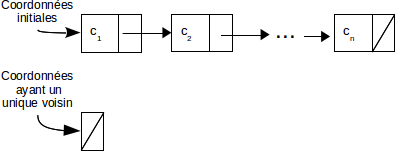
\includegraphics[scale=0.5]{solveur-listes}
      \caption{Valeur des listes au début de la résolution}
\end{figure}

La première liste contient toutes les coordonnées de la grille qui n'ont pas été traitées, tandis que la seconde liste contient les coordonnées qui auront été analysées par le «~tamisage~» mais dont on n'aura pas encore construit le chemin. Ainsi, après le tamisage, les listes seraient de la forme :

\begin{figure}[h]
      \centering
      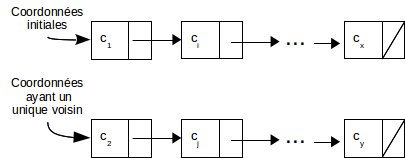
\includegraphics[scale=0.5]{solveur-listes2}
      \caption{Valeur des listes après tamisage}
\end{figure}

La partie construction, quant à elle, ne toucherait pas pas à la liste des coordonnées initiales mais modifierait la liste des coordonnées ayant un unique voisin, supprimant celles qui ont leurs chemins complétés.


\begin{figure}[h!]
      \centering
      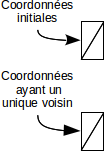
\includegraphics[scale=0.5]{solveur-listes3}
      \caption{Valeur des listes à la fin de la résolution}
\end{figure}

La résolution serait alors finie quand les deux listes seraient vides.

\subsection{Tamisage}

La partie tamisage du solveur serait principalement composé des fonctions de mise à jour des voisins dans le cas de coordonnées ayant un voisin unique ainsi que de la fonction qui teste s'il existe un chemin entre deux coordonnées.

La première partie du tamisage serait alors d'essayer, pour chaque coordonnées n'ayant qu'un unique voisin, de faire se répercuter ceci sur les autres coordonnées. 

\begin{algorithm}[H]
  \ForEach{coordonnées c \De la liste initiale}{
    \Si{$c$ n'a qu'un seul voisin}{
      $affecterVoisin(c,voisin de c,TabVoisins)$ \;
    }
  }
  \caption{Première partie du tamisage}
\end{algorithm}

La fonction \verb$affecterVoisin$ devrait ainsi également modifier la liste initiale, retirant les éléments modifiés et n'ayant plus qu'un unique voisin.

La seconde partie du tamisage consisterait, pour chaque couple de coordonnées supposées voisines, à tester si un chemin existe entre elles. Si ce n'est pas le cas, alors, on doit supprimer le lien de «~voisinage~» qui existe entre elles.

\begin{algorithm}[H]
  \ForEach{coordonnée $c$ \De la liste initiale}{
    \ForEach{coordonnée $c_2$ \De la liste des voisins de $c$}{
      \Si{NON($existeChemin(c,c_2,valeur de c,TabVoisins,NULL)$}{
        Retirer $c$ de la liste des voisins de $c_2$ \;
        Retirer $c_2$ de la liste des voisins de $c$ \;
      }
    }
  }
  \caption{Deuxième partie du tamisage}
\end{algorithm}

On pourra également après appeler affecterVoisin sur ces coordonnées dans le cas où, après retrait, il n'existerait plus qu'un seul voisin possible.

\subsection{Construction}

Dans cette partie, le solveur tenterait de créer des chemins ou, si un chemin complet n'est pas possible, des morceaux de chemins dans le but d'affiner le problème lors du tamisage suivant.

\begin{algorithm}[H]
  \ForEach{coordonnées $c$ \De la liste des coordonnées ayant un unique voisin}{
    consChemin($c$,voisin de $c$,valeur de $c$,TabVoisins) \;
  }
  \caption{Construction des chemins}
\end{algorithm}

La fonction \verb$consChemin$ devrait alors également modifier une liste du solveur. En effet, celle-ci devrait supprimer les coordonnées dont on a fini le chemin de la liste, ne laissant dedans que celles en attente de pouvoir progresser dans la construction du chemin.

\chapter{Manuel d'utilisation}

L'interface de l'éditeur est assez intuitive. Les boutons sont peu nombreux et les fonctionnalités moins utilisées sont dans la barre de menu.
Ce manuel liste la totalité des fonctionnalités du logiciel.

\section{Interaction}

\subsection{Barre de menu}


Les actions disponibles dans la barre de menu sont les suivantes :
\begin{itemize}
\item \emph{File...} : Ouvrir / Sauvegarder / Fermer
\item \emph{Edit...} : Indenter
\item \emph{Schéma...}
	\begin{itemize}
	\item \emph{Load schema file} : Ouvre un schéma et le lie automatiquement au fichier XML.
	\item \emph{Generate schema file} : Génère automatiquement un schéma à partir du fichier XML en utilisant les balises connues.
	\item \emph{Delete schéma} : Supprime la liaison entre le schéma et le fichier XML.
	\end{itemize}
\end{itemize}

\paragraph{}
Les actions Ouvrir, sauvegarder, indenter et valider sont disponibles en accès rapide sur la barre des boutons.

\subsection{Raccourcis}
\begin{itemize}
\item \emph{ctrl + o} : Ouvrir
\item \emph{ctrl + r} : Lancer la validation
\item \emph{ctrl + s} : Enregistrer 
\item \emph{ctrl + shift + s} : Enregistrer sous
\item \emph{ctrl + i} : Indenter automatiquement les lignes sélectionnées
\item \emph{F4} : Switch entre le fichier XML et le schéma
\end{itemize}

\section{Validation}
La validation permet de vérifier si le code XML entré est valide.
Il vérifie que les balises sont correctement formés (pas de balises croisés).
Et si un schéma est associé, le validateur vérifie que le fichier XML est bien en accord avec celui-ci.
En cas d'erreur, le message d'erreur est indiqué dans la console et le numéro de la ligne concernée est surligné en rouge.
Si la validation s'exécute correctement, la vue arborescence est générée.

\section{Vue arborescente}
Sur la vue arborescence il est possible de renommer un noeud (double clic), supprimer un noeud (clic droit / Supprimer), ou déplacer un noeud (glisser/déposer).
Lors d'une modification, la vue de l'éditeur de texte est automatiquement mise à jour.

\section{A propos du schéma}
L'association d'un schéma est une option du logiciel mais il n'est pas obligatoire de lier un schéma pour travailler un fichier XML.
Quand un schéma est ouvert, il est "lié" au fichier XML. La balise de lien vers le schéma est automatiquement ajoutée dans le fichier XML
et un enregistrement provoque la sauvegarde des deux fichiers (xml et schéma).
Lors de l'ouverture d'un fichier XML, le schéma est automatiquement ouvert si un chemin vers celui-ci est indiqué dans le XML.

\section{Fonctions du logiciel}


\begin{figure}[h!]
\noindent\makebox[\textwidth]{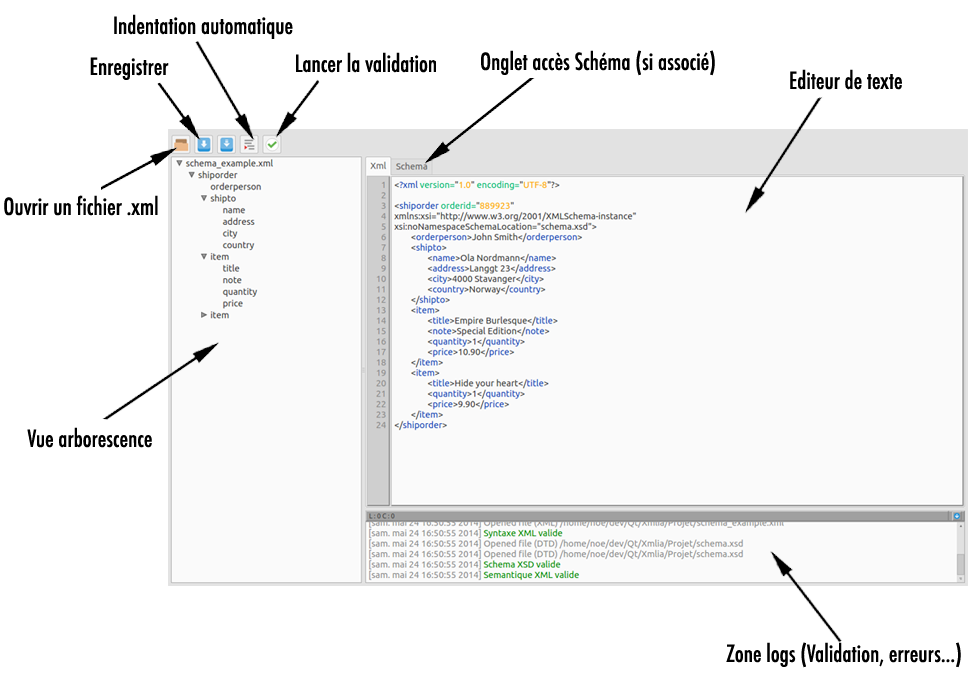
\includegraphics[width=450pt]{images/help1.png}}
\caption{Différentes sections du logiciel}
\end{figure}

\chapter{Perspectives et conclusions} 
  \section{Perspectives} 
 
Le solveur que nous avons élaboré peut-être amélioré de bien des manières.

Un des premiers ajouts que l'on peut imaginer est l'intégration de la génération de puzzle à partir d'une image, partie du sujet non traitée faute de temps et de personnes. Cet ajout pourrait permettre par la suite, éventuellement, la création d'un logiciel de jeu Link-Pix, proposant des grilles à résoudre qui ont été générées par le logiciel à partir d'image.

Un ajout plus «~simple~» serait la gestion des images de couleurs. En effet, on peut imaginer ajouter une caractéristique pour chaque case qui serait la couleur. La possibilité de lier deux indices serait ainsi dépendante de cette couleur, réduisant finalement le champ des possibilités. Une réécriture simple du code permettrait d'intégrer cet ajout.
 
  \section{Conclusions} 
   \subsection{Fonctionnement de l’application} 

   \subsubsection{Généralités}

Bien que notre solveur ait résolu les puzzles que nous lui avons proposés, nous n'avons pas la certitude qu'il puisse résoudre tous les puzzles à solution unique. Ainsi, nous construisons les débuts de chemins dont nous sommes certains, mais nous n'analysons pas si d'autres portions de chemins, situées non pas en début mais au milieu, sont sûres.

\begin{figure}[h!]
      \centering
      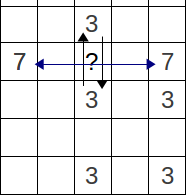
\includegraphics[scale=0.5]{solvable1}
      \caption{On ne peut pas construire de façon sûre les débuts du chemin qui relie les 7, mais il passe forcément entre les deux 3, ce qui peut réduire les possibilités de voisinage.}
\end{figure}

En outre, notre solveur a été testé sur des puzzles de tailles raisonnables, et nous ne pouvons pas savoir avec certitude si les performances sur de plus gros puzzles seront identiques.
Cela dit, le solveur fonctionne sur les problèmes auquels nous l'avons soumis, et il semble efficace tant en utilisation mémoire qu'en temps de calcul.

Ainsi, malgré les problèmes d'organisation que nous avons eu, nous avons atteint notre objectif qui était de fournir un solveur opérationnel, et nous avons même pu créer une interface graphique, alors que nous ne pensions pas en avoir le temps.

\subsubsection{Choix des outils}

Le langage choisi pour développer ce projet, le langage C, aurait sans doute pu être remplacé par un langage de plus haut niveau, ce qui nous aurait permis un développement plus rapide, nous affranchissant ainsi des problèmes de gestion de mémoire. C'était cependant le langage le mieux connu de tous les membres de l'équipe, ce qui nous a permis de travailler plus facilement en groupe.

L'utilisation du gestionnaire de version Git nous a permis de travailler plus facilement à distance, peut-être au détriment de réunions de travail qui auraient pu être plus fréquentes. De même, du retard a été pris suite à certains oublis de soumission, faisant que la version en ligne n'était pas la plus à jour. Il s'est quand même globalement avéré être un outil de choix et a efficacement soutenu notre projet du début à la fin, nous aidant ainsi énormément.

L'utilisation du générateur de documentation Doxygen fut aussi positive. En effet, cet outil s'est avéré facile à utiliser et relativement puissant, nous fournissant ainsi une documentation claire. Nous avions ainsi accès aux caractéristiques d'une fonction beaucoup plus aisément que dans une recherche directement dans le code source.
 
   \subsection{Fonctionnement du groupe de travail} 
 
Les démarrages du projet ont été difficiles, notamment dû au fait que certains membres de l'équipe n'assistaient pas aux réunions. Nous avons ainsi pris du retard au début, les choix ne parvenant pas à être fixés dû aux manques de rigueur des absents.

Cela dit, au milieu du semestre, le retrait complet des étudiants inactifs sur le projet nous a permis de nous mettre au travail en groupe, de façon relativement efficace. Seule une semaine relativement chargée en contrôles nous a fait baisser d'intensité de travail, mais nous avons de façon globale eu un travail assez régulier, jusqu'à la fin où nous avons eu un rythme un peu plus élevé afin d'essayer de terminer dans les temps.

Au final, nous avons réussi à nous entendre, travaillant ensemble et en s'entraidant, de sorte que nous avons pu être relativement efficaces. Les erreurs trouvées étaient rapidement corrigées, notamment grâce à l'utilisation de Git, et nous avons pris du plaisir à travailler ensemble.


\appendix

\chapter{Documents d’analyse}

\begin{figure}[h]
  \centering
  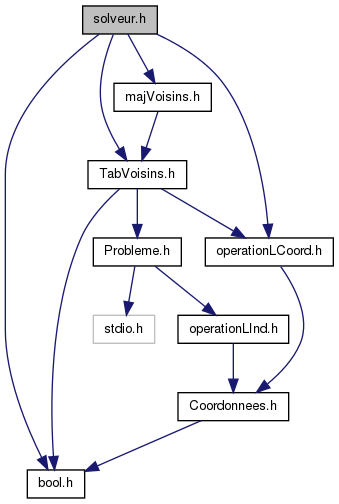
\includegraphics[scale=0.5]{solveur-dependance}
  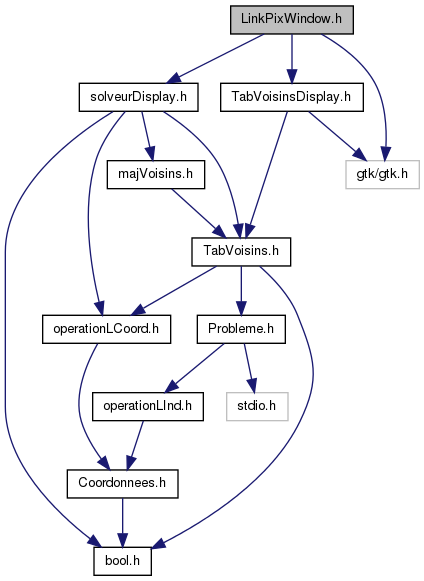
\includegraphics[scale=0.5]{link-pix-window-dependance}
  \caption{Graphe des dépendances du solveur à gauche et de du solveur graphique à droite}
  \label{graphes-dependance}
\end{figure}

Les fichiers \verb$solveur.h$ et \verb$solveur.c$ ne sont pas utilisés dans le cadre du logiciel, mais sont conservés car ils contiennent le solveur en un seul morceau (et non pas des itérations découpées comme dans \verb$solveurDisplay.h$ et \verb$solveurDisplay.c$, qui sont des adaptations du solveur pour la surcouche graphique).

\input{manuel-de-reference.tex}
\chapter{Listing}
\section{Coordonnees.c}
\lstinputlisting{../Coordonnees.c}
\section{LinkPixWindow.c}
\lstinputlisting{../LinkPixWindow.c}
\section{Probleme.c}
\lstinputlisting{../Probleme.c}
\section{TabVoisins.c}
\lstinputlisting{../TabVoisins.c}
\section{TabVoisinsDisplay.c}
\lstinputlisting{../TabVoisinsDisplay.c}
\section{main.c}
\lstinputlisting{../main.c}
\section{majVoisins.c}
\lstinputlisting{../majVoisins.c}
\section{operationLCoord.c}
\lstinputlisting{../operationLCoord.c}
\section{operationLInd.c}
\lstinputlisting{../operationLInd.c}
\section{solveur.c}
\lstinputlisting{../solveur.c}
\section{solveurDisplay.c}
\lstinputlisting{../solveurDisplay.c}


\end{document}
